\documentclass[11pt]{article}

\usepackage[margin=1in]{geometry}
\usepackage{graphicx}
\usepackage{booktabs}
\usepackage{amsmath}
\usepackage{amssymb}
\usepackage{caption}
\usepackage{float}
\usepackage[hidelinks]{hyperref}
\usepackage{xcolor}

\graphicspath{{figs/}}
\captionsetup{font=small}
\newcommand{\vadv}{v_{\mathrm{adv}}}
\newcommand{\opin}{\omega_{\mathrm{pin}}}

\title{\textbf{A Data-Driven Reduced-Order Model for Friction-Stir Welding}\\[2pt]
\large POD/SVD Feasibility: Density Fields and Particle Clouds}
\author{FSW--ROM study (JAXTrace)}
\date{\today}

\begin{document}
\maketitle

\begin{abstract}
We assess whether a reduced-order model (ROM) can predict the full 3D
outcome of a friction-stir-welding (FSW) simulation from two process
inputs --- advance velocity $\vadv$ (\texttt{INLET\_VELOCITY}) and pin
rotation $\opin$ (\texttt{PIN\_RPM}) --- using linear Proper Orthogonal
Decomposition (POD) via the SVD. Two output targets are studied: the
Eulerian mean-density field and the Lagrangian particle cloud. The
manifold of responses is \emph{curved} (intrinsic dimension ${\sim}2.5$
below ${\sim}10$ linear modes for 90\% energy), so linear POD is a
\emph{convenient first approximation, not a fitted model} of the geometry.
With only 20 cases the density surrogate reaches ${\sim}28\%$ held-out
error (per-case spread $18$--$43\%$), and this error has \emph{two}
non-negligible parts: a ${\sim}10$--14\% linear-POD \emph{basis} error (the
singular spectrum has no elbow --- the curved ensemble is not low-rank in a
linear basis) plus the additional \emph{regression} error, the latter most
simply explained by degrees-of-freedom starvation (fitting ${\sim}7$--10
mode coefficients from 20 points). Two representation choices
reduce the error --- the \emph{time-averaged} density beats a single final
snapshot, and a \emph{2D $(y,z)$ cross-section} reaches ${\sim}21\%$ (with
the caveat that it also predicts a lower-information target). Curvature and
active-subspace diagnostics are \emph{suggestive but not conclusive at
$n{=}20$}: they hint that the error concentrates on the sampling boundary
(extrapolation) rather than in high-curvature interior regions, but the
correlations rest on ${\sim}20$ noisy LOOCV estimates and cannot separate
this from ``too few samples, period.'' The unambiguous, method-independent
conclusion is that \textbf{more samples are required} --- particularly to
extend and densify the sampling envelope and to resolve where the curvature
changes --- both to lower the linear-POD error and to \emph{unlock}
nonlinear alternatives (patch/local POD, manifold learning, autoencoders)
that 20 points cannot currently support.
\end{abstract}

\tableofcontents

%======================================================================
\section{Dataset}
%======================================================================
Twenty full-order FSW simulations on a Latin-hypercube-like sampling of
$(\vadv,\opin)$, with $\vadv\in[5.0,10.0]\times10^{-3}$~m/s and
$\opin\in[-800,-400]$~RPM. Authoritative parameters come from each case's
\texttt{run\_jaxtrace.sh} (the CSV \texttt{dt} column is inconsistent and
was not used). A notable design property: $\vadv\cdot t_{\max}=\vadv\cdot
\mathrm{DT}\cdot N_{\mathrm{STEPS}}=0.075$ for \emph{every} case --- the
runs are length-matched, so all cases advect the same total distance.

\begin{table}[H]\centering
\begin{tabular}{lll}
\toprule
 & density study & particle study \\
\midrule
snapshot & one static 3D \texttt{mean\_density} field & final-step displacement of 360k particles \\
cases used & 20 & 20 \\
source & \texttt{particles\_union\_density.vtkhdf} & \texttt{particles.vtkhdf} \\
\bottomrule
\end{tabular}
\caption{The two ROM targets. Both use all 20 cases after data-quality
fixes (Sec.~\ref{sec:rerun}).}
\end{table}

%======================================================================
\section{Method: pre-SVD preparation, SVD, and validation}
%======================================================================

\paragraph{Correspondence (pre-SVD).}
POD needs every snapshot as a vector on \emph{one shared grid}, so that
``column $j$'' means the same thing in every case. The native density
grids differ per case (extent/spacing scale with $\vadv$), so every case
is trilinearly resampled onto a common intersection-box grid, then a
boundary margin is trimmed (1 voxel per wall, 6 off $z_{\max}$ to remove
an artificial top-layer). For particles, the seeds are byte-identical
across cases (same 360k particles, same \texttt{ParticleID} order), so
correspondence is free: a per-particle displacement stacks directly.

\paragraph{SVD (method of snapshots).}
The snapshot matrix $X\in\mathbb{R}^{n\times m}$ is short and fat
($n=20$ cases, $m\sim10^6$ voxels). We mean-centre and factor the small
Gram matrix $G=X_cX_c^{\top}\in\mathbb{R}^{n\times n}$ with
\texttt{jax.numpy.linalg.svd}, recovering the spatial modes; this is
identical to the economy SVD of $X_c$ but avoids GPU \texttt{gesvd}
failures on the wide matrix. The per-voxel mean is the POD reference
field (``mode 0''); optional normalizations (global scalar, per-case
$L^2$/mass, $\log$) were tested but change little (Sec.~\ref{sec:results}).

\paragraph{Validation: projection vs.\ LOOCV.}
Two error numbers appear throughout and must not be conflated.
\emph{Projection error} fits POD on all cases and reconstructs case $i$
from its \emph{own} coefficients --- it isolates the \emph{basis} error
(what linear POD cannot represent even with perfect coefficients). For
density it is ${\sim}14\%$ at $K{=}7$ and still ${\sim}10\%$ at $K{=}10$
(90\% energy) --- \emph{not} negligible. \emph{Leave-one-out
cross-validation} (LOOCV) is the real generalization test: for each case
$i$, fit POD on the other $n{-}1$, fit a regressor
$(\vadv,\opin)\mapsto$ mode coefficients on them, predict the held-out
coefficients, reconstruct, and measure relative $L^2$ error:
\[
\hat\rho_i=\bar\rho+\sum_{k=1}^{K}\hat A_{ik}\,\phi_k,\qquad
e_i=\frac{\lVert\hat\rho_i-\rho_i\rVert}{\lVert\rho_i\rVert}.
\]
A surrogate cannot project an unseen field, so LOOCV necessarily tests
\emph{POD + regression together}. The total held-out error
(${\sim}28\%$) thus has \emph{two} substantial components: a
${\sim}10$--14\% \textbf{basis} error (the linear POD does not fit the
curved ensemble well --- see the absence of a spectral elbow below) plus
the additional regression error on top. Neither component is small; both
trace back to the same cause (a curved manifold under-sampled by 20
points). Three lightweight regressors are compared: \texttt{rbf}
(thin-plate spline), \texttt{gp} (small NumPy Gaussian process),
\texttt{poly} (degree-2).

%======================================================================
\section{Core results}\label{sec:results}
%======================================================================

\subsection{Density field}
The singular-value spectrum decays \emph{gently, with no elbow at all}
(consecutive ratios $\sigma_k/\sigma_1 = 1.00, 0.61, 0.53, 0.43, 0.41,
0.33,\ldots$ --- a smooth taper, not a knee): 90\% energy needs ${\sim}10$
modes and the coverage curve keeps climbing with diminishing returns. This
is itself a negative result for linear POD: the field ensemble is
\emph{not} low-rank-linear, so there is no natural truncation $K$ and even
the best $K$ leaves a non-trivial basis error (Sec.~2.5). This is the
expected fingerprint of a transport-dominated / high-Kolmogorov-width
problem (density blobs shifted by $\vadv$ are nearly $L^2$-orthogonal).
Normalization barely moves the held-out error. LOOCV is ${\sim}28\%$
(rbf); the error concentrates in the high-$|\opin|$/low-$\vadv$ corner and
at the sampling convex-hull edges. Restricting to the near-pin first 20\%
of $x$ (dropping the $\vadv$-sensitive wake) improves the surrogate.

\begin{figure}[H]\centering
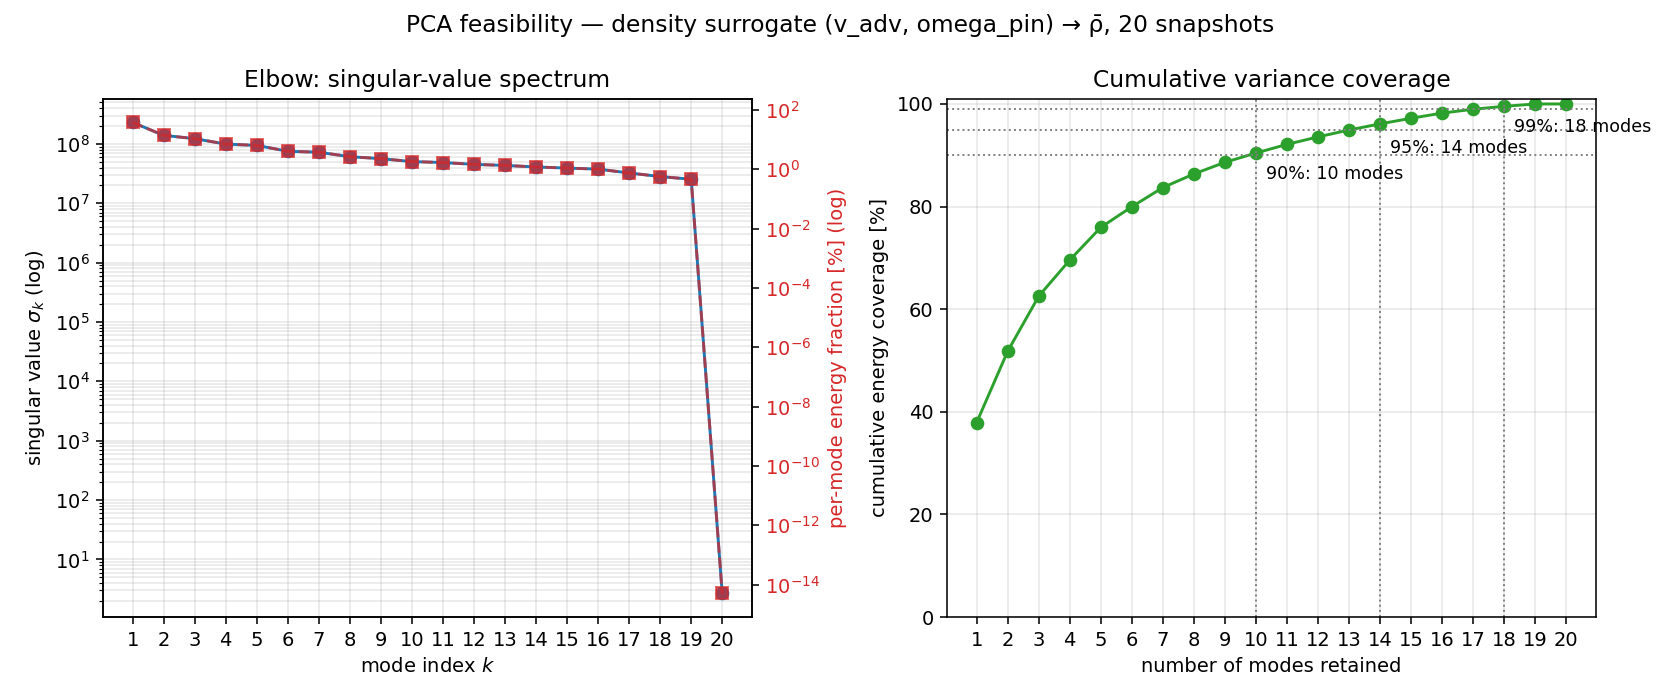
\includegraphics[width=\linewidth]{rom_pca_elbow_coverage.png}
\caption{Density POD spectrum. Left: singular-value elbow (mode 17 is the
null mode from mean-centring). Right: cumulative energy coverage, with
90/95/99\% thresholds annotated.}
\end{figure}

\begin{figure}[H]\centering
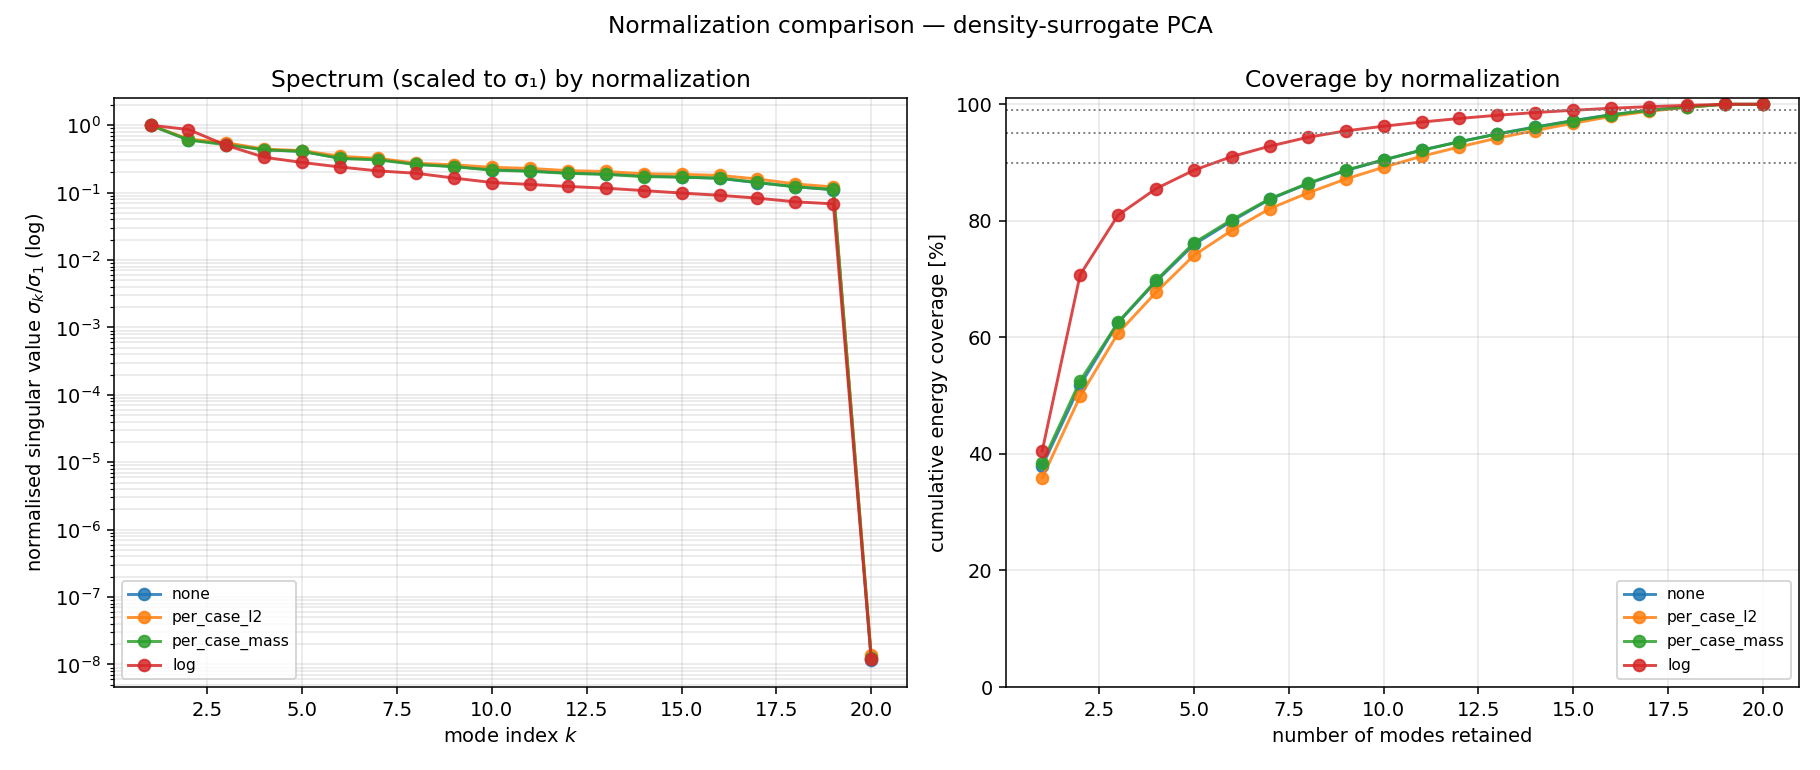
\includegraphics[width=\linewidth]{rom_pca_normalize_compare.png}
\caption{Normalization comparison. \texttt{per\_case} options barely change
the spectrum; \texttt{log} reaches coverage in fewer modes but its error
is measured in log-density space and is not comparable.}
\end{figure}

\begin{figure}[H]\centering
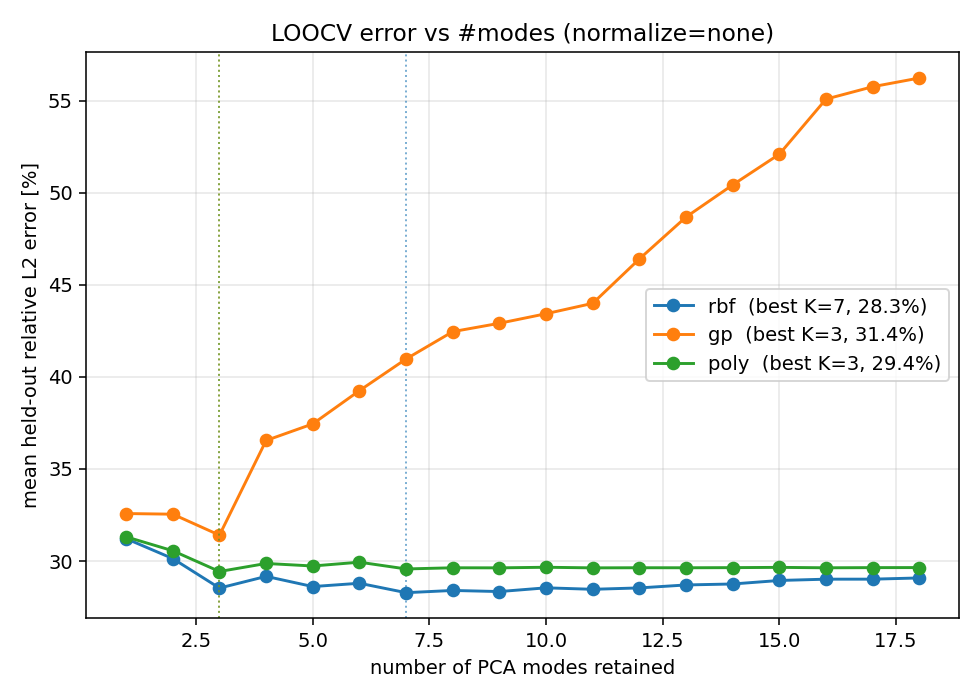
\includegraphics[width=0.88\linewidth]{rom_loocv_error_vs_modes.png}
\caption{Density LOOCV error vs.\ number of retained modes, per regressor.
The dip (bias/variance sweet spot) is at $K\approx3$--7; all reasonable
regressors converge to a similar floor set by the sample count.}
\end{figure}

\begin{figure}[H]\centering
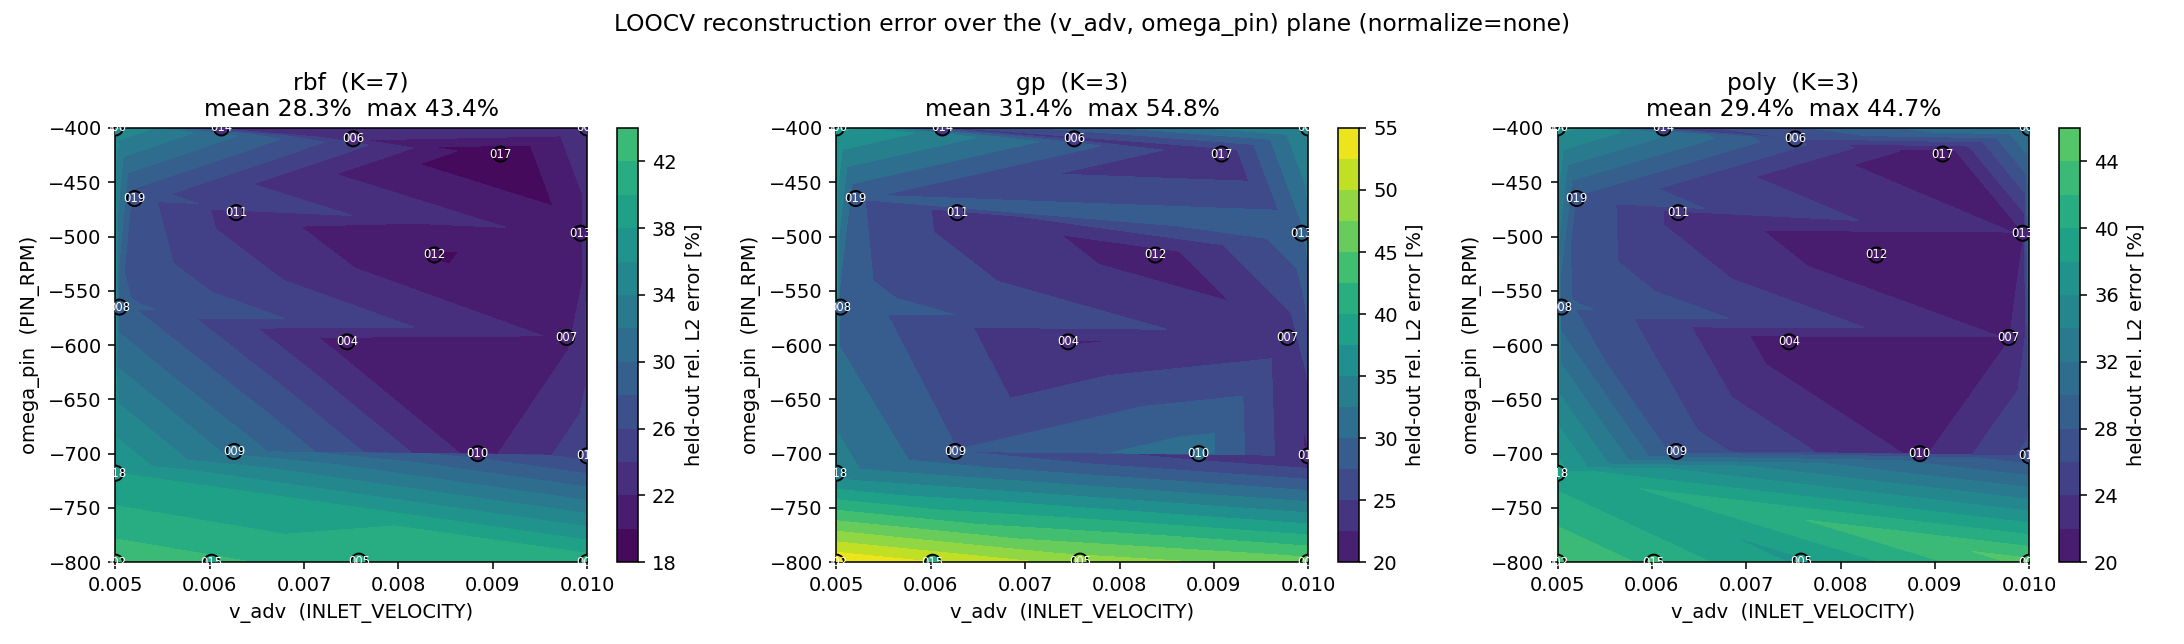
\includegraphics[width=\linewidth]{rom_loocv_error_maps.png}
\caption{Density held-out error over the $(\vadv,\opin)$ plane. Error peaks
in the high-$|\opin|$/low-$\vadv$ corner --- the sparsely sampled region.}
\end{figure}

\subsection{Particle cloud}
Seeds are byte-identical across cases, so the natural target is the
per-particle final-step displacement. A subtle finding: because
correspondence is exact, subtracting the (constant) bulk drift is a rigid
offset fully absorbed by mean-centring, so raw / co-moving / final
representations give \emph{identical} POD modes. Thresholding to
``eliminate unaffected particles'' is moot: $>97\%$ of particles exceed
even $|\xi|>5\Delta p$, since the seed spacing is tiny relative to typical
displacement.

\begin{figure}[H]\centering
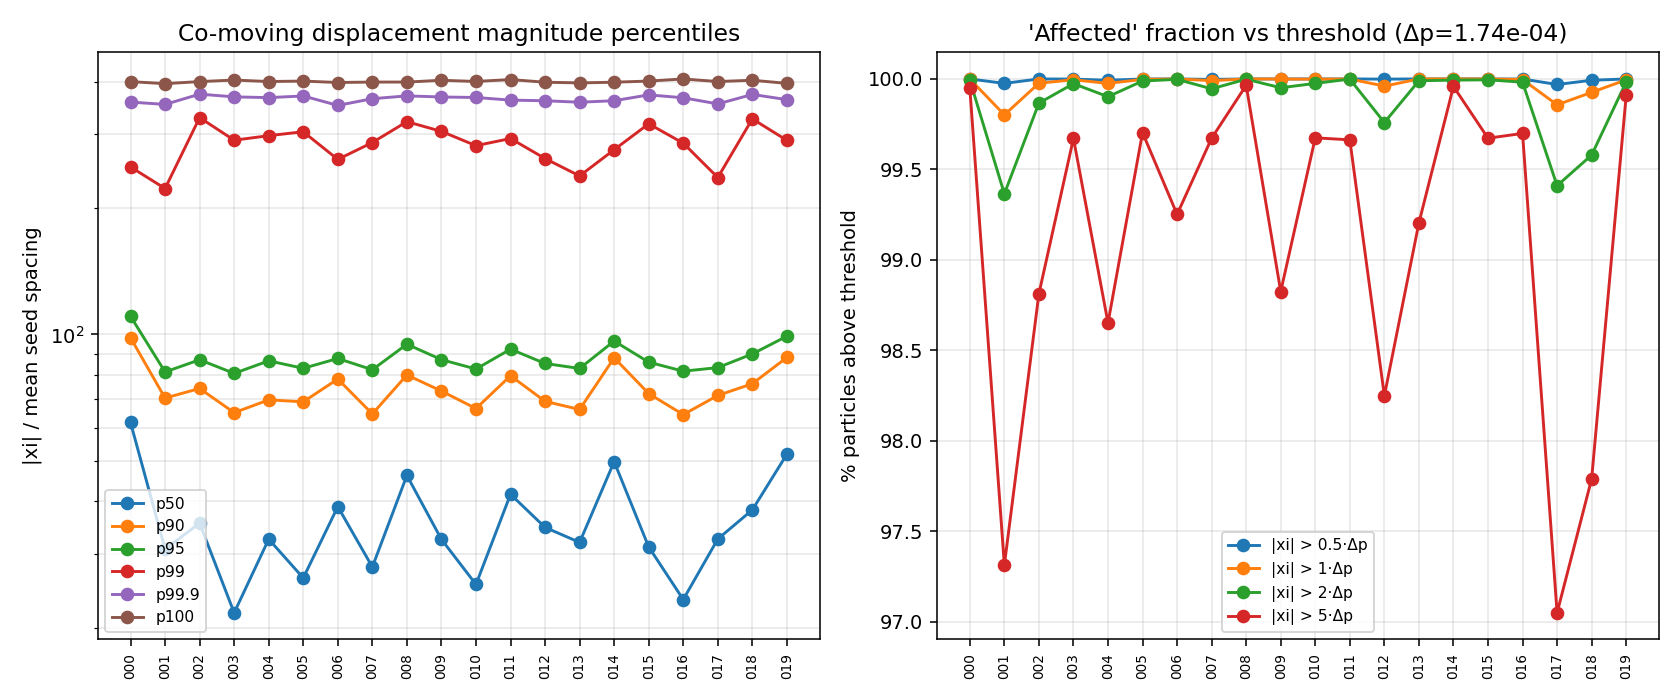
\includegraphics[width=0.92\linewidth]{rom_particles_displacement_stats.png}
\caption{Co-moving displacement magnitude $|\xi|/\Delta p$ per case (left)
and the ``affected'' fraction vs.\ threshold (right). Almost all particles
are ``affected'', so a magnitude threshold cannot isolate the stir zone.}
\end{figure}

\begin{figure}[H]\centering
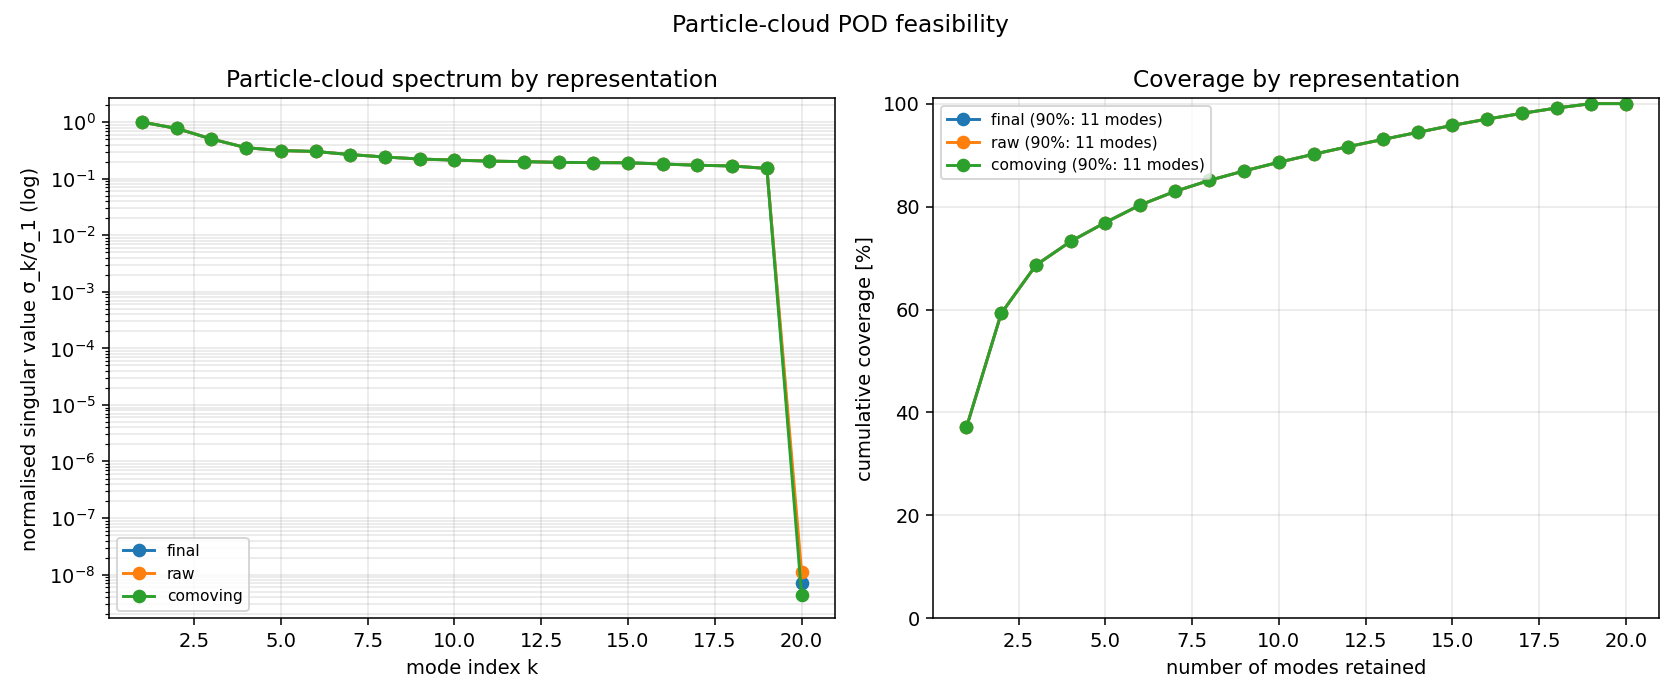
\includegraphics[width=\linewidth]{rom_particles_elbow_compare.png}
\caption{Particle-cloud POD by representation. The \texttt{final},
\texttt{raw}, and \texttt{comoving} curves coincide exactly --- drift
subtraction does not change the modes.}
\end{figure}

\begin{figure}[H]\centering
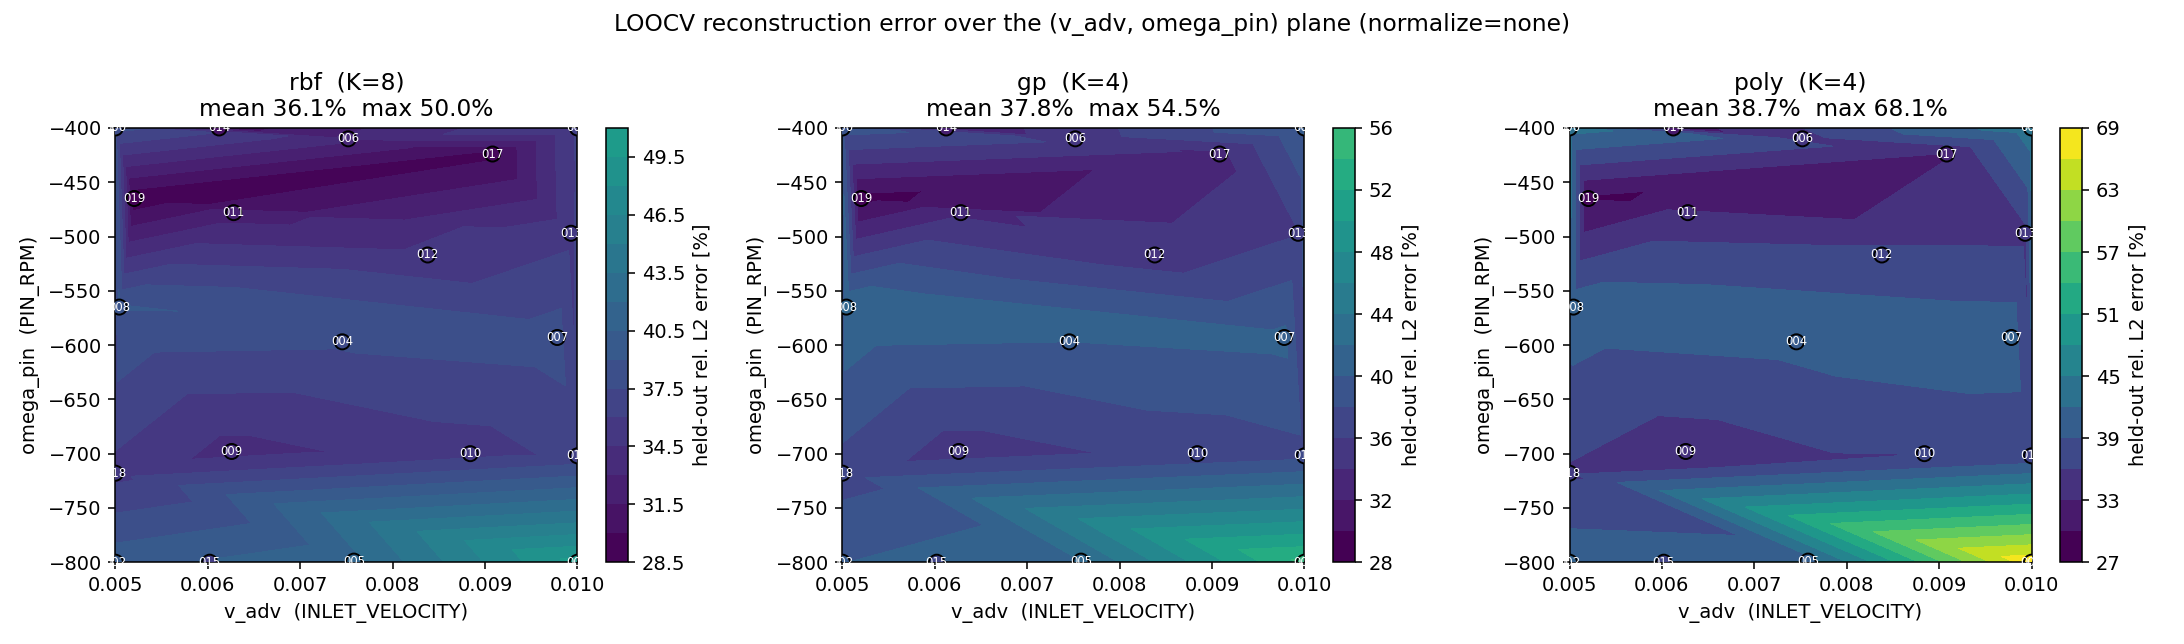
\includegraphics[width=\linewidth]{rom_particles_loocv_error_maps_comoving.png}
\caption{Particle displacement LOOCV error over the $(\vadv,\opin)$ plane.}
\end{figure}

The Lagrangian displacement is harder to predict than the Eulerian
density (${\sim}36\%$ vs.\ ${\sim}28\%$ LOOCV), consistent with the
literature: a density field spatially averages many trajectories and is a
lower-variance, more predictable quantity.

%======================================================================
\section{Why the error is what it is: three diagnostics}
%======================================================================

\subsection{Input features and active subspace}
Mapping the inputs to physics-motivated features --- weld pitch
$p_w=\vadv/|\opin|$, $\log$ inputs, and the first-stage ROM (velocity /
temperature / pressure) coefficients --- \emph{none} beat the raw
two-scalar baseline. An active-subspace analysis is consistent with this:
the estimated input$\to$coefficient map is \emph{apparently} low-rank, with
its dominant direction close to \emph{pure $\vadv$} rather than weld pitch
--- so if a reduction to one input combination were warranted it would be
$\vadv$, not $p_w$. We caution, however, that at $n{=}20$ over a 2D input
space an ``apparently 1D'' active subspace cannot be cleanly distinguished
from simply having too few samples to resolve the second direction's
effect; small-sample regressions generically look artificially low-rank.
The first-stage coefficients are largely a reparametrisation of the two
scalars (leading modes have $R^2\approx1.0$ with the inputs; only mode
$\geq3$ carries new information, which does not drive the density modes),
and adding all of them overfits.

\begin{figure}[H]\centering
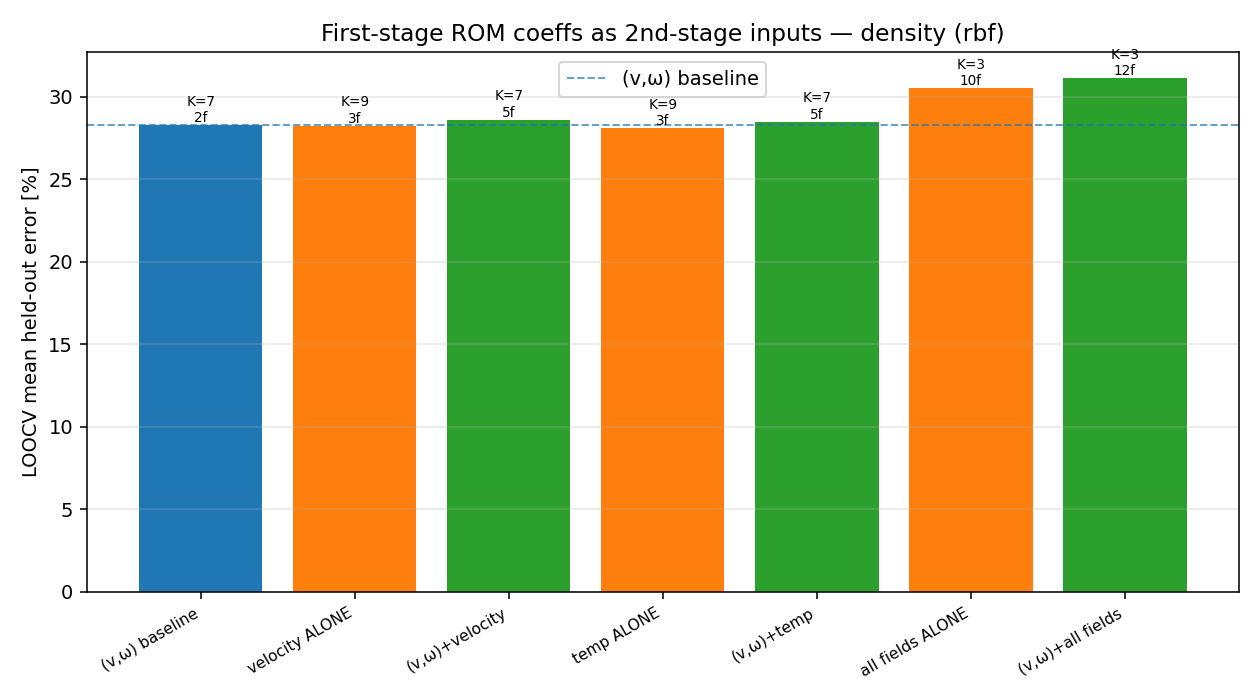
\includegraphics[width=0.85\linewidth]{rom_firststage_density.png}
\caption{First-stage ROM coefficients as second-stage inputs. Velocity
coefficients alone are marginal; piling on all fields overfits
(12 features, 20 points $\Rightarrow$ best-$K$ collapses to 3).}
\end{figure}

\subsection{Manifold geometry}
Characterising the case manifold with linear/metric methods (before any
nonlinear embedding) reveals a \emph{high linear dimension but low
intrinsic dimension} --- the signature of a smooth but \emph{curved}
manifold. Classical MDS axes are the variance-ordered principal directions
of the case cloud; we measure their alignment with the inputs afterwards.

\begin{figure}[H]\centering
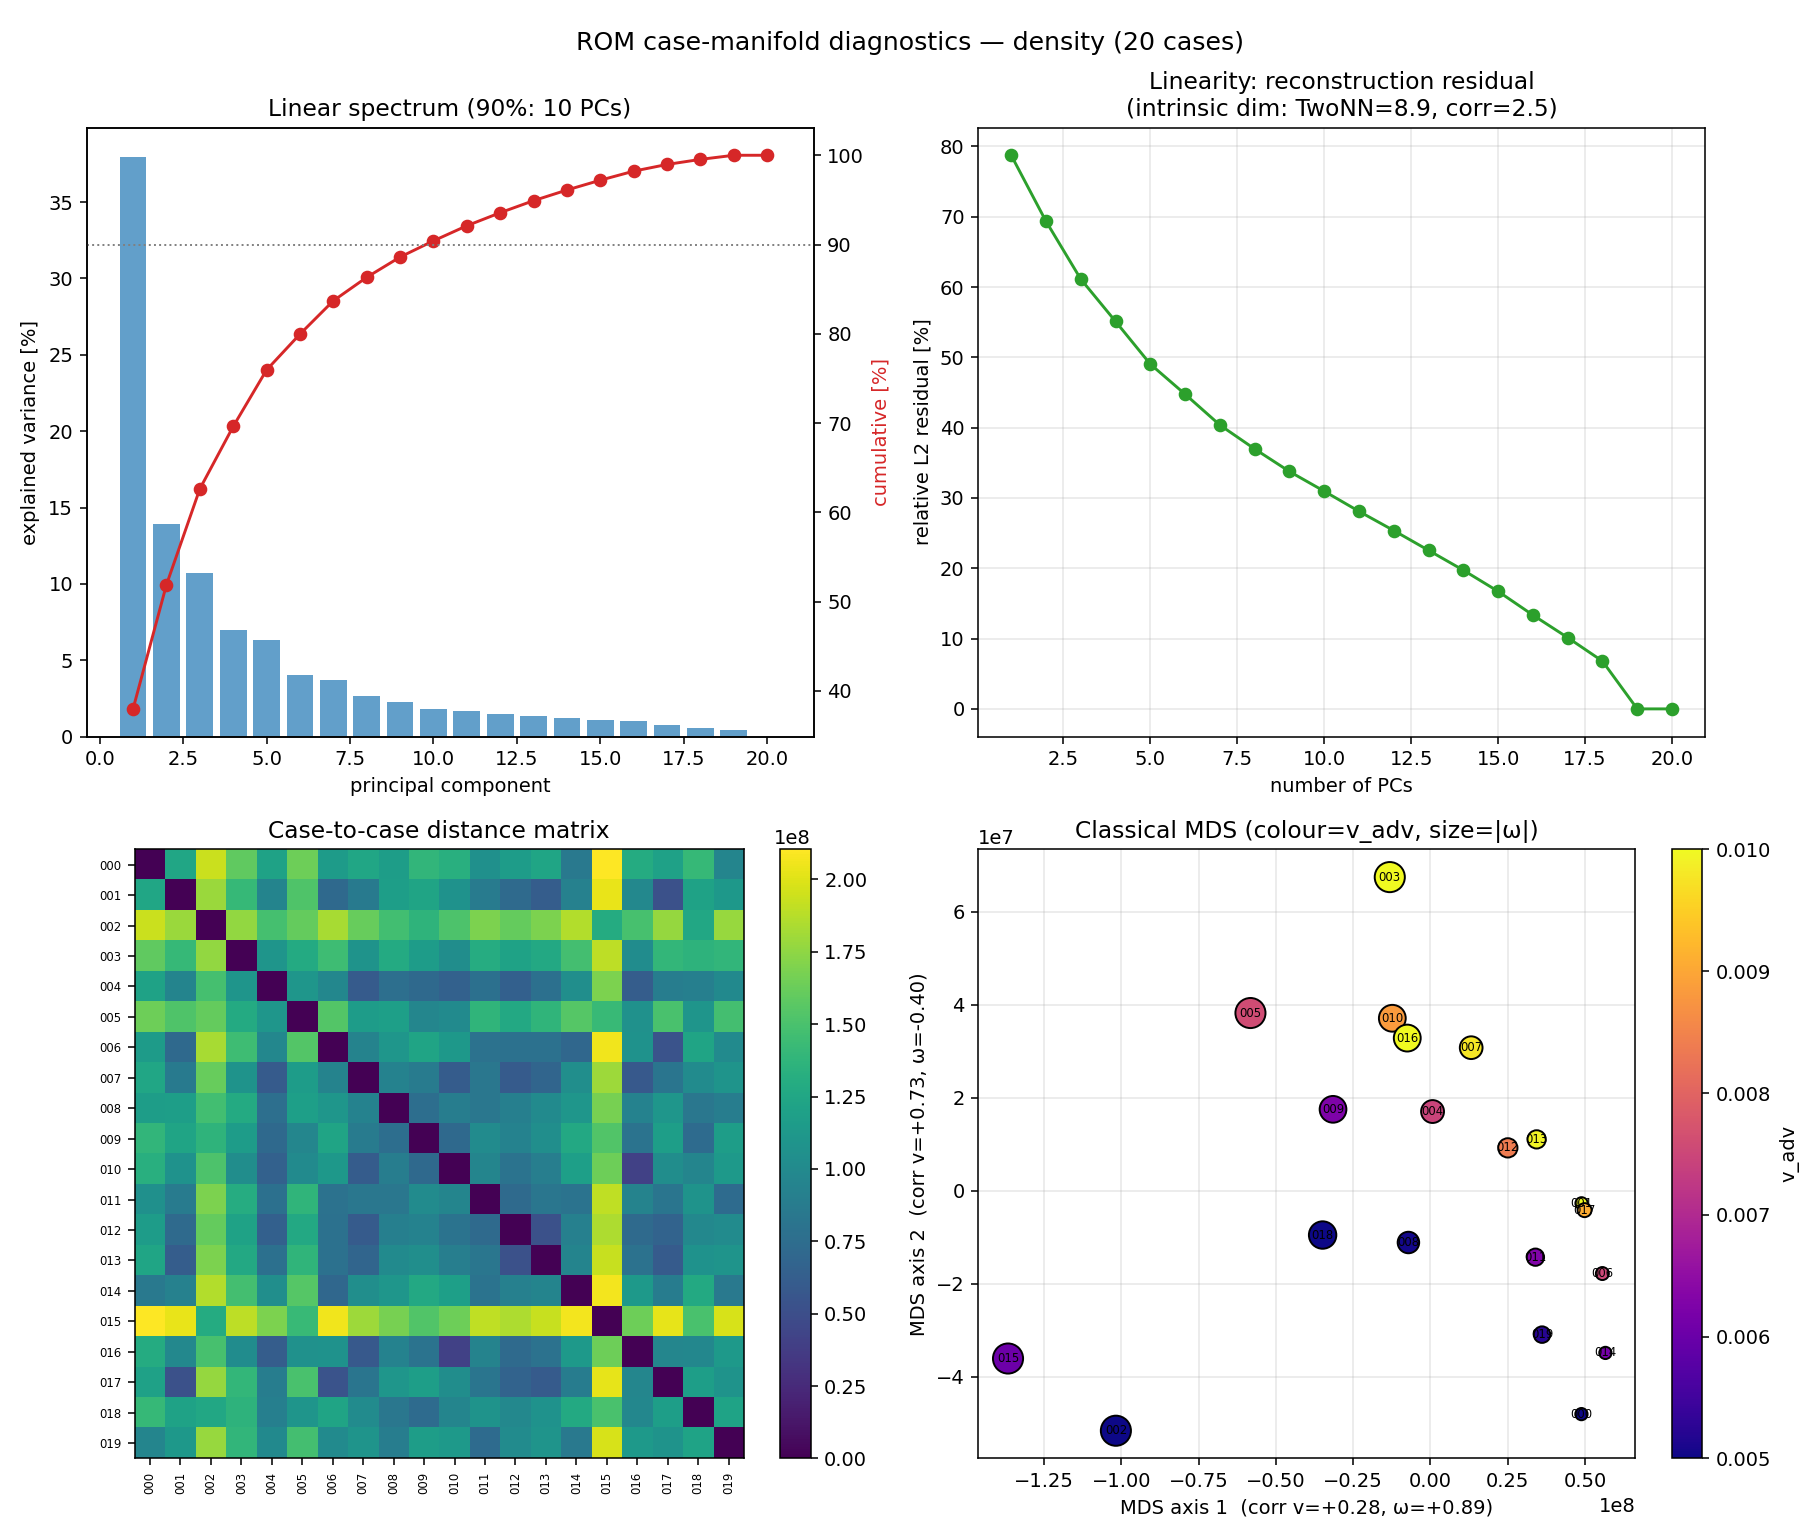
\includegraphics[width=0.9\linewidth]{rom_manifold_density.png}
\caption{Density case-manifold diagnostics: spectrum, linearity residual,
distance matrix, and classical-MDS layout coloured by $\vadv$ / sized by
$|\opin|$. Intrinsic dim ${\approx}2.5$ vs.\ 10 linear PCs for 90\%.}
\end{figure}

\begin{figure}[H]\centering
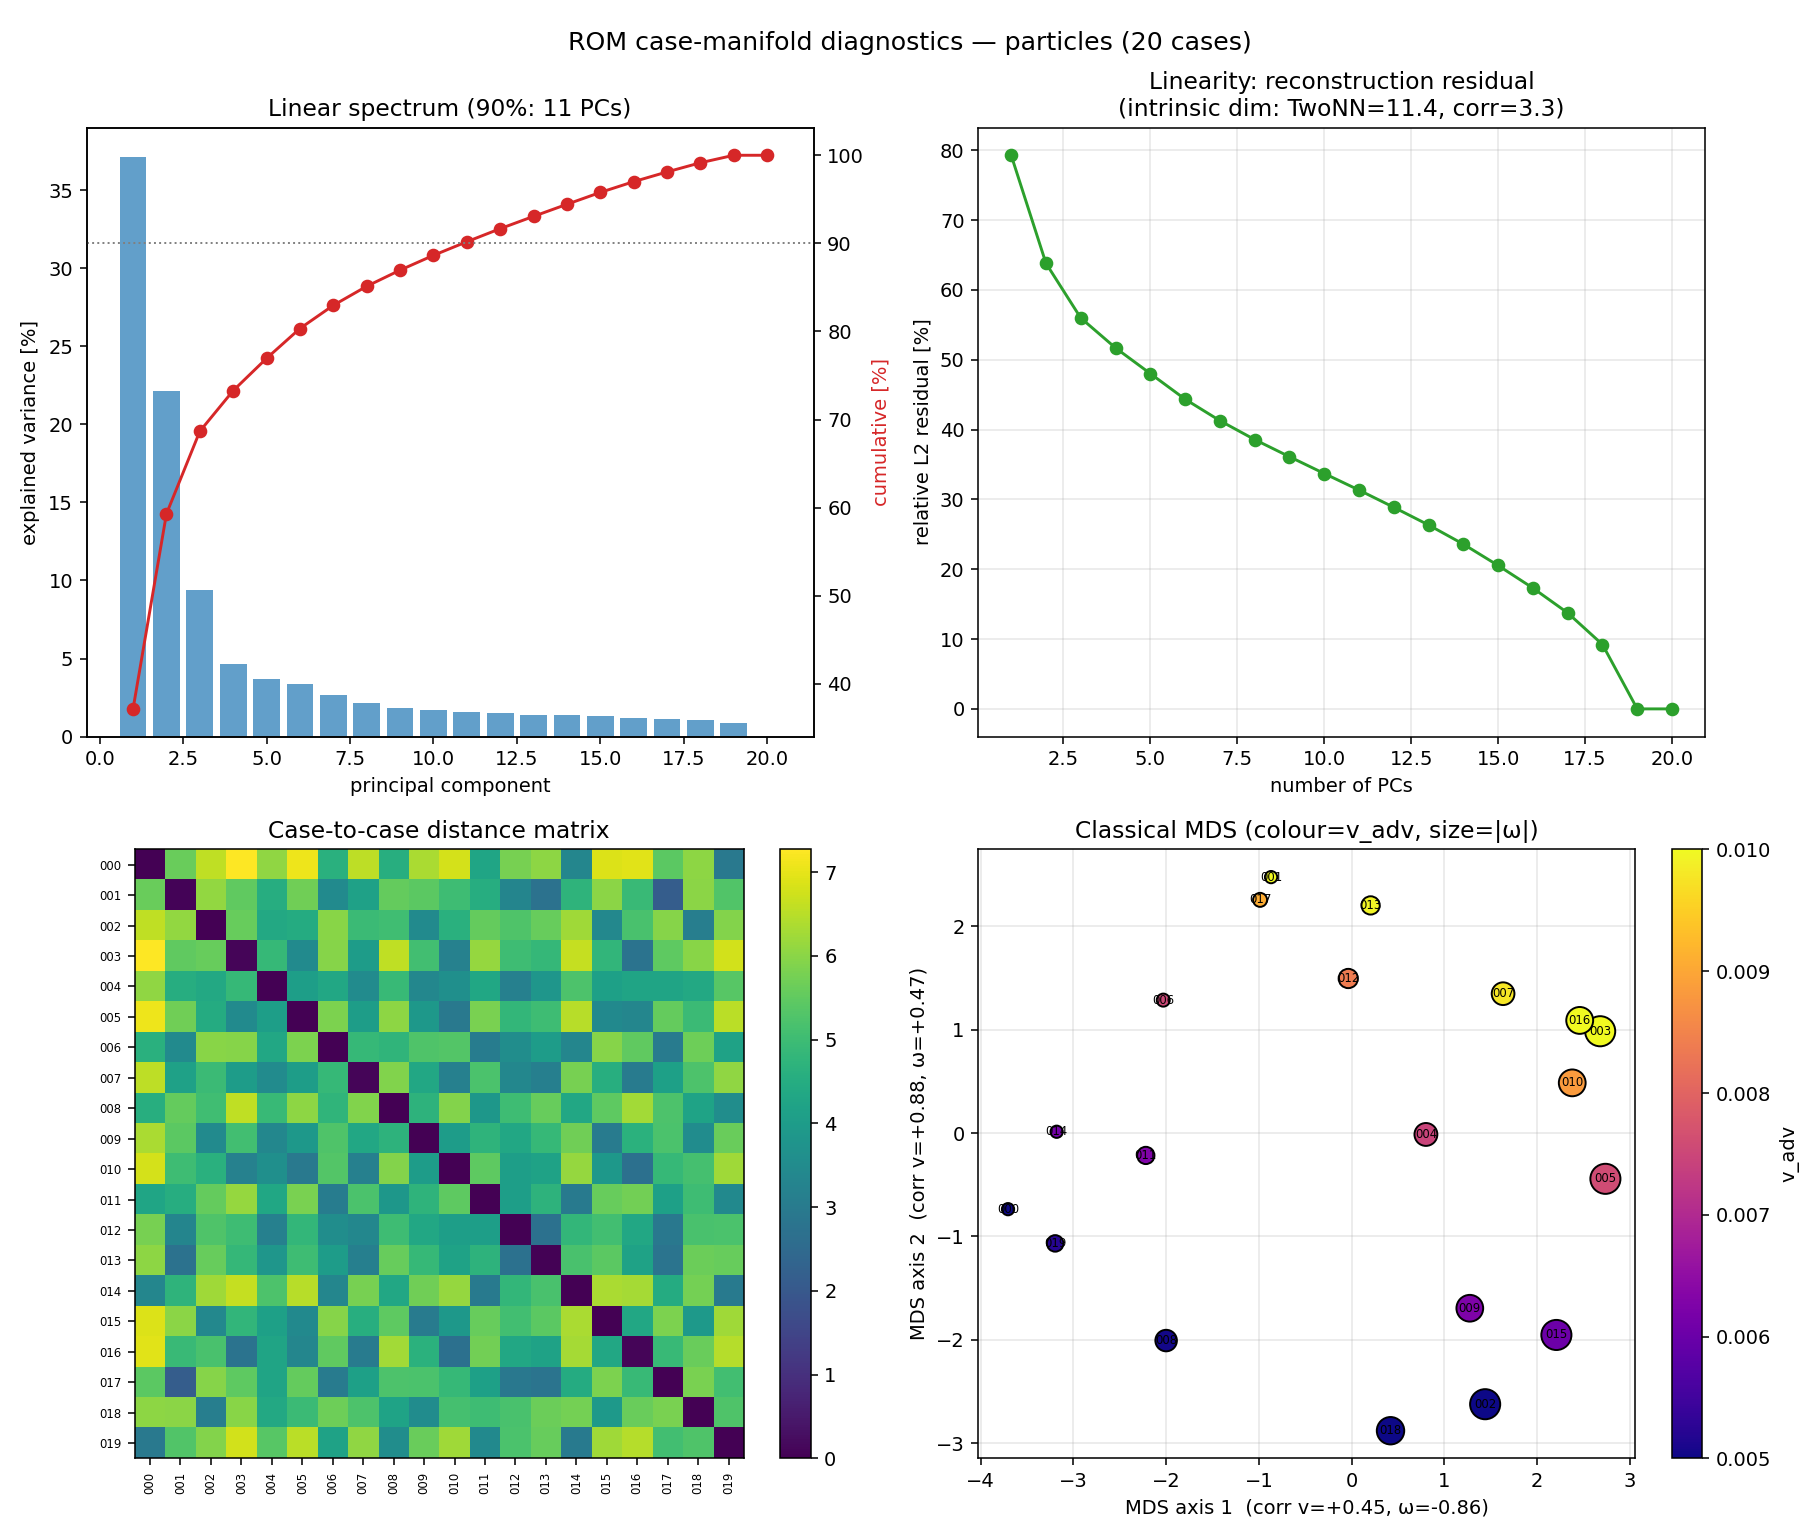
\includegraphics[width=0.9\linewidth]{rom_manifold_particles.png}
\caption{Particle case-manifold diagnostics. MDS axis~1 tracks $\opin$
strongly; particles give a clean $(\opin,\vadv)$ split, whereas density's
axis~2 mixes the parameters (the wake couples them).}
\end{figure}

\paragraph{How the MDS axes arise, and why they differ.}
Classical MDS double-centres the distance matrix,
$B=-\tfrac12 J D^2 J$, and takes coordinates $x_i=\sqrt{\lambda_i}\,v_i$
for the two largest eigenvalues --- so the axes are variance-ordered and
data-driven (for Euclidean $D$ this is PCA of the cases), \emph{not}
parameter-picked. Both targets have \textbf{axis~1 $\approx\opin$} (the
largest source of case-to-case variation). Particles split cleanly
(axis~2 $\approx$ pure $\vadv$); density's axis~2 \emph{mixes} $\vadv$ and
$\opin$ because the field couples them through the wake (length $\propto
\vadv$, pattern $\propto\opin$). A small negative MDS eigenvalue is the
expected mild-curvature signal.

\subsection{Discrete curvature: how curved, and where}\label{sec:curv}
The intrinsic-dimension gap above says the manifold \emph{is} curved; to
see \emph{how much} and \emph{where}, we compute discrete secant-vector
curvature directly in the high-dimensional snapshot space (not the MDS
embedding). Three estimators are used: the \textbf{turning angle} between
consecutive secants along 1D parameter paths (fix one input, sweep the
other); the \textbf{Menger curvature}
$\kappa=4\,\mathrm{Area}/(abc)=1/R_{\mathrm{circ}}$ of consecutive triples,
scale-normalised by the median pairwise distance so it is dimensionless
and comparable across manifolds; and a \textbf{local-PCA} curvature
(trailing $k$-NN eigenvalue energy beyond the intrinsic dimension). The
estimators were validated on known geometry (a straight line gives $0$; a
circle of radius $R$ gives Menger $=1/R$ exactly).

\begin{figure}[H]\centering
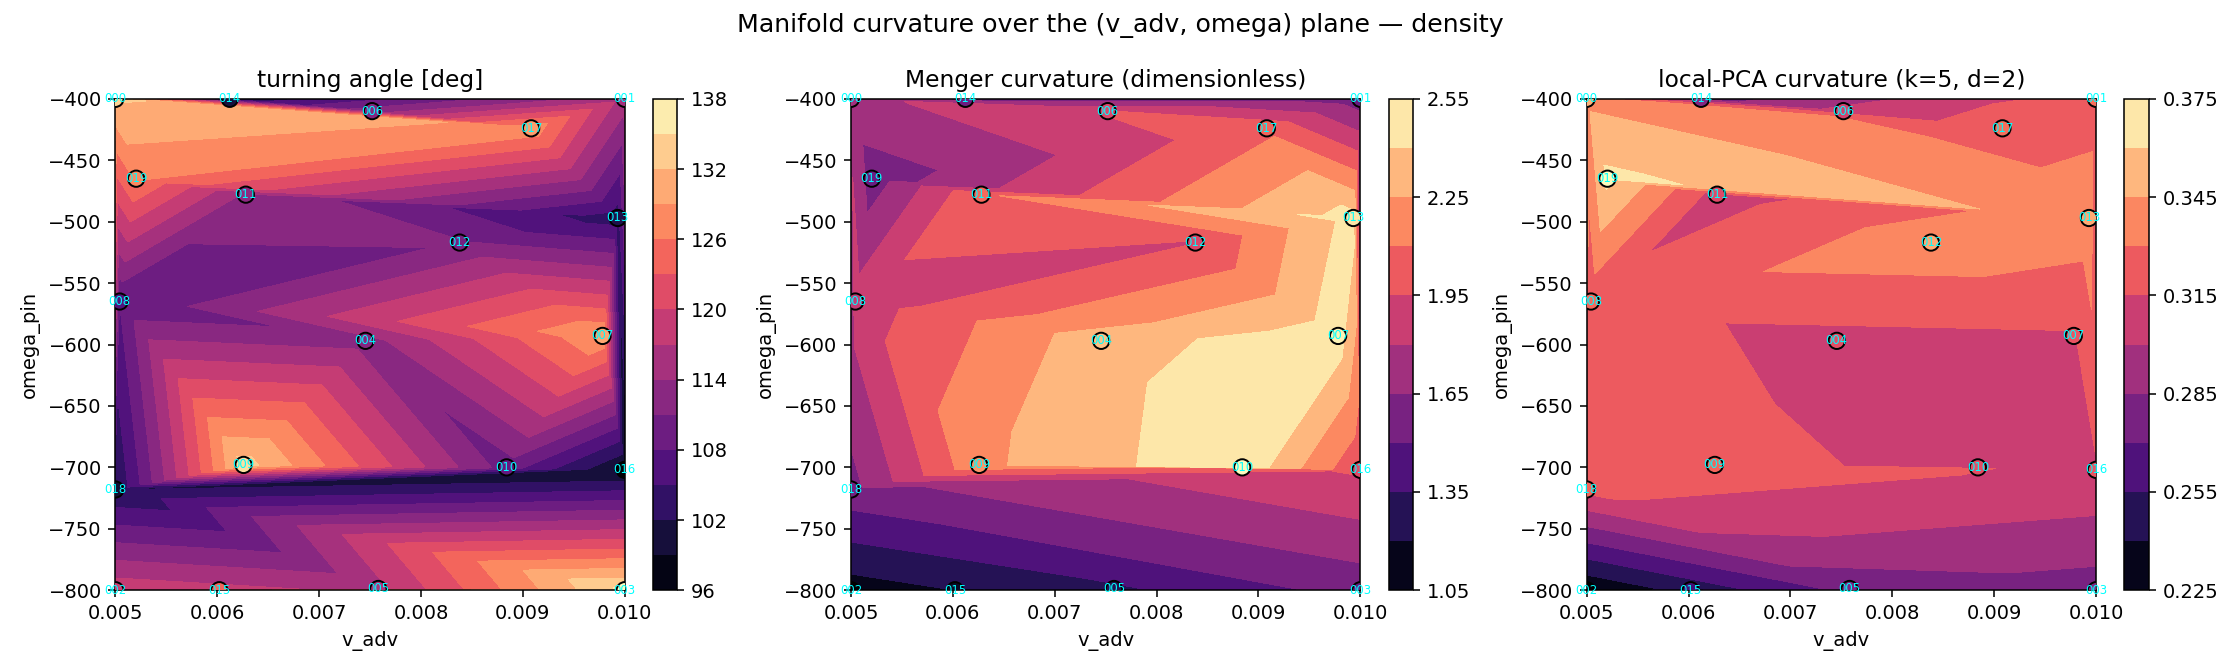
\includegraphics[width=\linewidth]{rom_curvature_density.png}
\caption{Density manifold curvature over the $(\vadv,\opin)$ plane
(turning angle, Menger, local-PCA). Curvature is \emph{highest in the
interior} (mid/high $\vadv$) and \emph{lowest along the $\opin=-800$
sampling edge}.}\label{fig:curv}
\end{figure}

One observation is robust; a second is only suggestive.
\begin{itemize}
\item \textbf{(Robust) The manifold is smooth, not sharply bent.} Turning
angles sit at ${\sim}117^\circ$ for every target --- the honest
high-dimensional signature that consecutive secants are near-orthogonal;
there are no sharp folds. Scale-normalised Menger is ${\sim}1.7$--$1.9$
across all four representations (density/particle, 3D/2D), i.e.\ comparable
and moderate. This says the response varies smoothly with the inputs ---
good for interpolation, and an argument \emph{against} the presence of
discontinuities that only a nonlinear method could handle.
\item \textbf{(Suggestive) Error appears to concentrate on the sampling
boundary.} Per-case LOOCV error correlates \emph{negatively} with Menger
($-0.74$) and local-PCA ($-0.58$) curvature: the highest-error cases
(\texttt{002}, \texttt{003}, \texttt{005}, \texttt{015}, all at
$\opin\approx-800$) sit on the convex-hull boundary and have \emph{low}
curvature, while the lowest-error cases are interior and most curved
(Fig.~\ref{fig:curv}). We deliberately do \emph{not} treat this as an
established mechanism: both the curvature correlation and the per-case
LOOCV error are computed from ${\sim}20$ points, and LOOCV error is itself
a high-variance, single-held-out estimate (here the per-case error spans
$18$--$43\%$). A correlation of $-0.74$ on 20 noisy points has wide
sampling uncertainty, and the pattern is equally consistent with the
simpler ``too few samples, period.'' The local-PCA estimator's
cross-manifold ranking is unreliable at $n{=}20$ (used only for the
within-manifold pattern).
\end{itemize}

\paragraph{Interpretation (a hypothesis, not a diagnosis).} The most
\emph{parsimonious} explanation of the projection-vs-LOOCV gap is
degrees-of-freedom starvation: retaining ${\sim}7$--10 modes leaves only
${\sim}10$--13 effective DOF for the regression, fitted from 20 points ---
a very thin margin that alone predicts large held-out error. On top of
that, the geometry \emph{hints} that the residual error is worst where the
model must extrapolate past the sampling boundary rather than in
high-curvature interior regions. Both readings point the same practical
way (more, better-placed samples), so we adopt the recommendation without
committing to the curvature-based causal story as fact.

\subsection{The bottleneck}
The total ${\sim}28\%$ error is limited on \emph{two} fronts. First, the
linear POD \textbf{basis} itself is inadequate: the spectrum has no elbow
and the projection (own-coefficient) error is ${\sim}10$--14\% at usable
$K$, because the transport-dominated ensemble is not low-rank in a linear
basis. Second, the \textbf{regression} adds error on top, most simply from
\textbf{degrees-of-freedom starvation}: 20 samples cannot robustly fit
${\sim}7$--10 mode coefficients plus the interpolation between them.
Consistent with this, no lever that does \emph{not} add information
helps --- normalization, input features, and regressor choice all converge
to a similar floor, and every LOOCV number carries a standard error of
order a few percentage points (e.g.\ density $28.3\%$ has per-case spread
$18$--$43\%$), so the point estimates in the tables should be read as
${\pm}$ several points, not exact. The suggestive boundary/curvature
pattern (Sec.~\ref{sec:curv}) refines \emph{where} to add samples but is
not needed for the core conclusion: both the basis inadequacy and the
regression starvation stem from \textbf{too few samples of a curved
response}, and both improve only with more data.

%======================================================================
\section{Data-quality fixes (all 20 cases)}\label{sec:rerun}
%======================================================================
Three cases were initially set aside and later fixed, after which the
entire study runs on all 20. Cases \texttt{000}/\texttt{001} produced
${\sim}1.4$--$2.5\%$ \emph{runaway particles} (flying to $x\approx2$--3.7~m
vs.\ a ${\sim}0.08$~m domain); the density driver sized its voxel grid
from the trajectory bbox, which those runaways inflated to $10^{11}$--
$10^{12}$ voxels $\Rightarrow$ GPU out-of-memory. A clean rerun (plus an
absolute physical ROI box) removed them. Case \texttt{002}'s density had
been \emph{host}-RAM OOM-killed (batch dedup over 8001 steps $\times$ 360k
particles $\approx2.9$~billion points $>$ 58~GiB); recomputing with a step
stride fixed it. Including the (now clean) cases barely moved any number,
confirming the earlier exclusions did not bias the study.

%======================================================================
\section{Representation studies}
%======================================================================

\subsection{Final-step vs.\ union (time-averaged) density}
The core density study uses the \emph{union} density (time-average over
the whole trajectory). Computing instead a \emph{final-step} density (one
snapshot) and re-running the suite shows the union is markedly better for
ROM (Table~\ref{tab:finalstep}). Temporal averaging denoises the
case-to-case stochastic variability of any single instant, so the union
field varies more smoothly and lower-dimensionally with the inputs.

\begin{table}[H]\centering
\begin{tabular}{lcc}
\toprule
metric & union (time-avg) & final-step \\
\midrule
PCA modes for 90\% & \textbf{10} & 12 \\
PC-1 energy & \textbf{37.9\%} & 25.5\% \\
LOOCV, full domain (rbf) & \textbf{28.3\%} & 49.3\% \\
LOOCV, near-pin (rbf) & \textbf{24.6\%} & 75.2\% \\
manifold intrinsic dim & \textbf{2.5} & 4.8 \\
\bottomrule
\end{tabular}
\caption{Union density is substantially more predictable than a single
final snapshot.}\label{tab:finalstep}
\end{table}

\begin{figure}[H]\centering
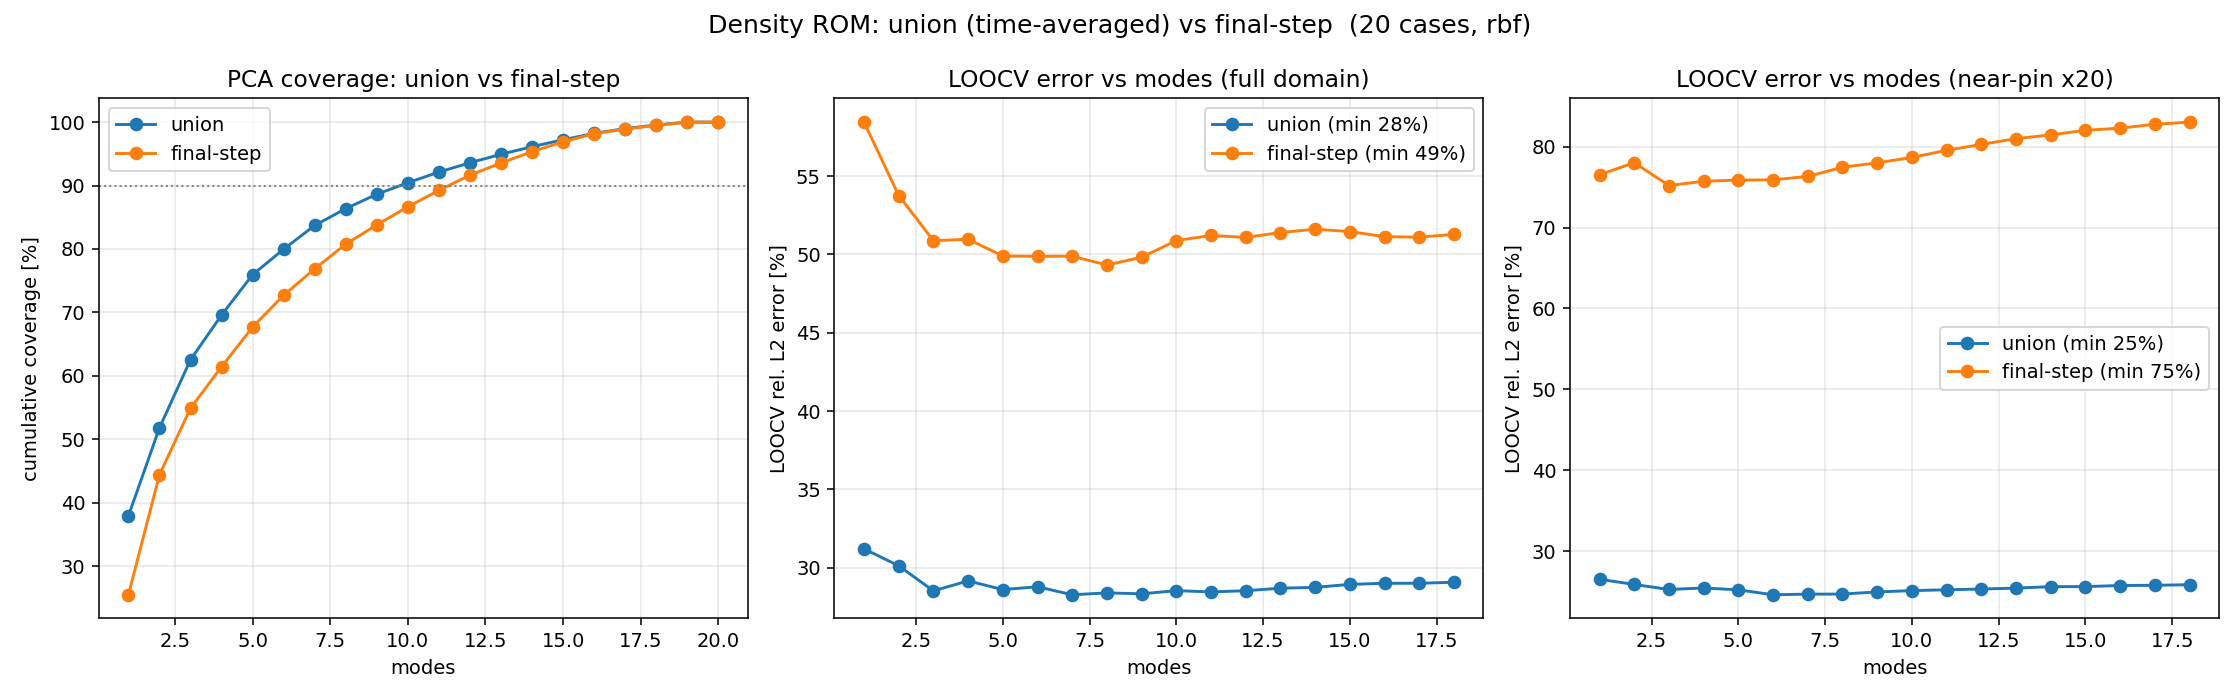
\includegraphics[width=\linewidth]{rom_density_union_vs_finalstep.png}
\caption{Union vs.\ final-step density: coverage curves (left) and LOOCV
error vs.\ modes for the full domain (centre) and near-pin (right).}
\end{figure}

\subsection{2D $(y,z)$ cross-section (collapse the advection axis)}
The wake stretches along $x$ and its \emph{length} scales with $\vadv$ ---
the very feature that dominates the error. Collapsing $x$ (summing the
slab into a $(y,z)$ cross-section, a ${\sim}300\times$ reduction) tests
whether integrating out that axis helps. It \textbf{helps density and
hurts particles}, for the same underlying reason (Table~\ref{tab:2d}).

\begin{table}[H]\centering
\begin{tabular}{lcc}
\toprule
 & 3D & 2D $(y,z)$ \\
\midrule
density --- PCA modes for 90\% & 10 & \textbf{6} \\
density --- LOOCV (rbf) & 28.3\% & \textbf{20.6\%} \\
density --- intrinsic dim & 2.5 & \textbf{1.7} \\
particles --- PCA modes for 90\% & 11 & 14 \\
particles --- LOOCV (rbf) & 36.1\% & 41.4\% \\
particles --- intrinsic dim & 3.3 & 4.3 \\
\bottomrule
\end{tabular}
\caption{2D cross-section: the best density result of the study, but worse
for particles.}\label{tab:2d}
\end{table}

\begin{figure}[H]\centering
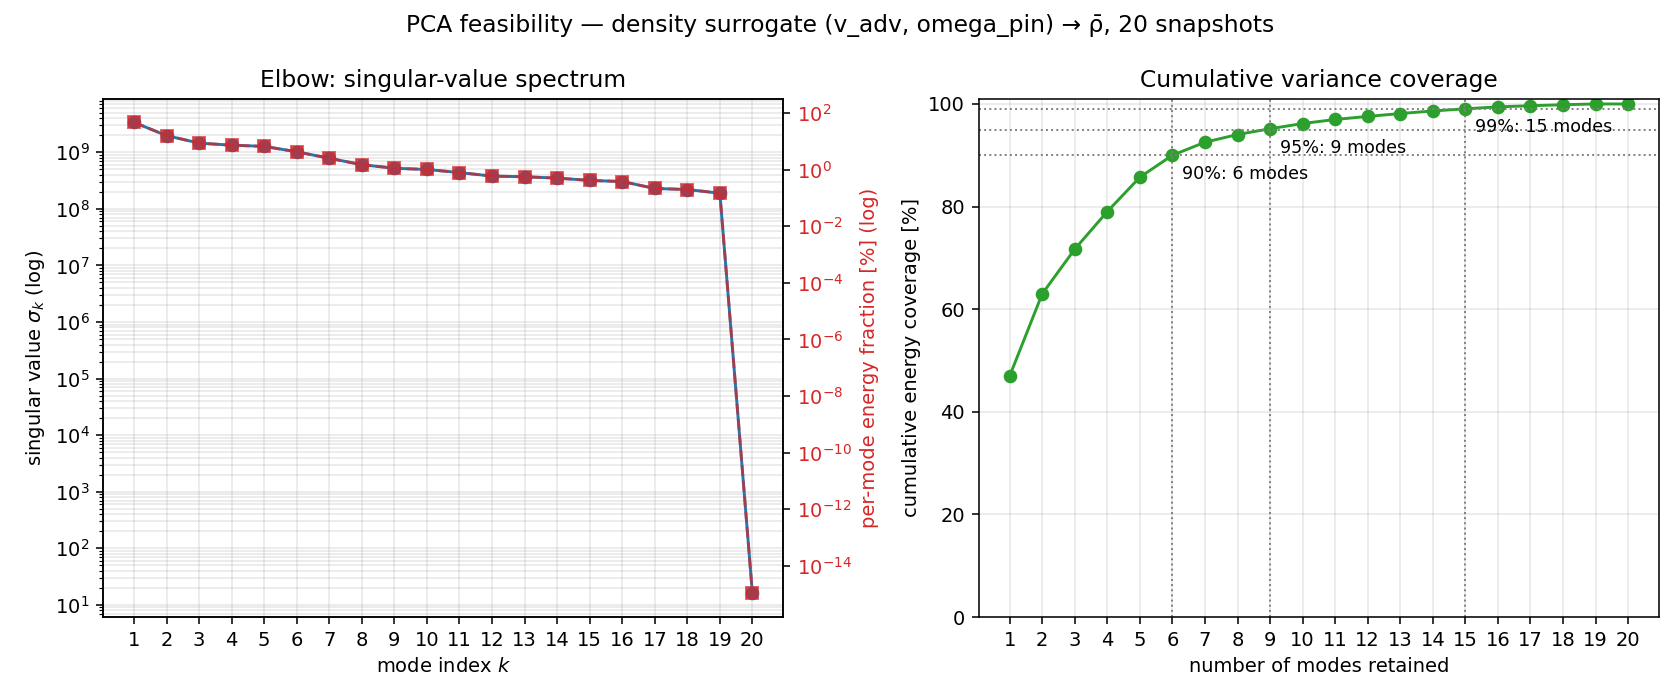
\includegraphics[width=\linewidth]{rom_pca_elbow_coverage_2d.png}
\caption{2D density POD spectrum --- markedly faster decay than 3D
(90\% in 6 modes).}
\end{figure}

\begin{figure}[H]\centering
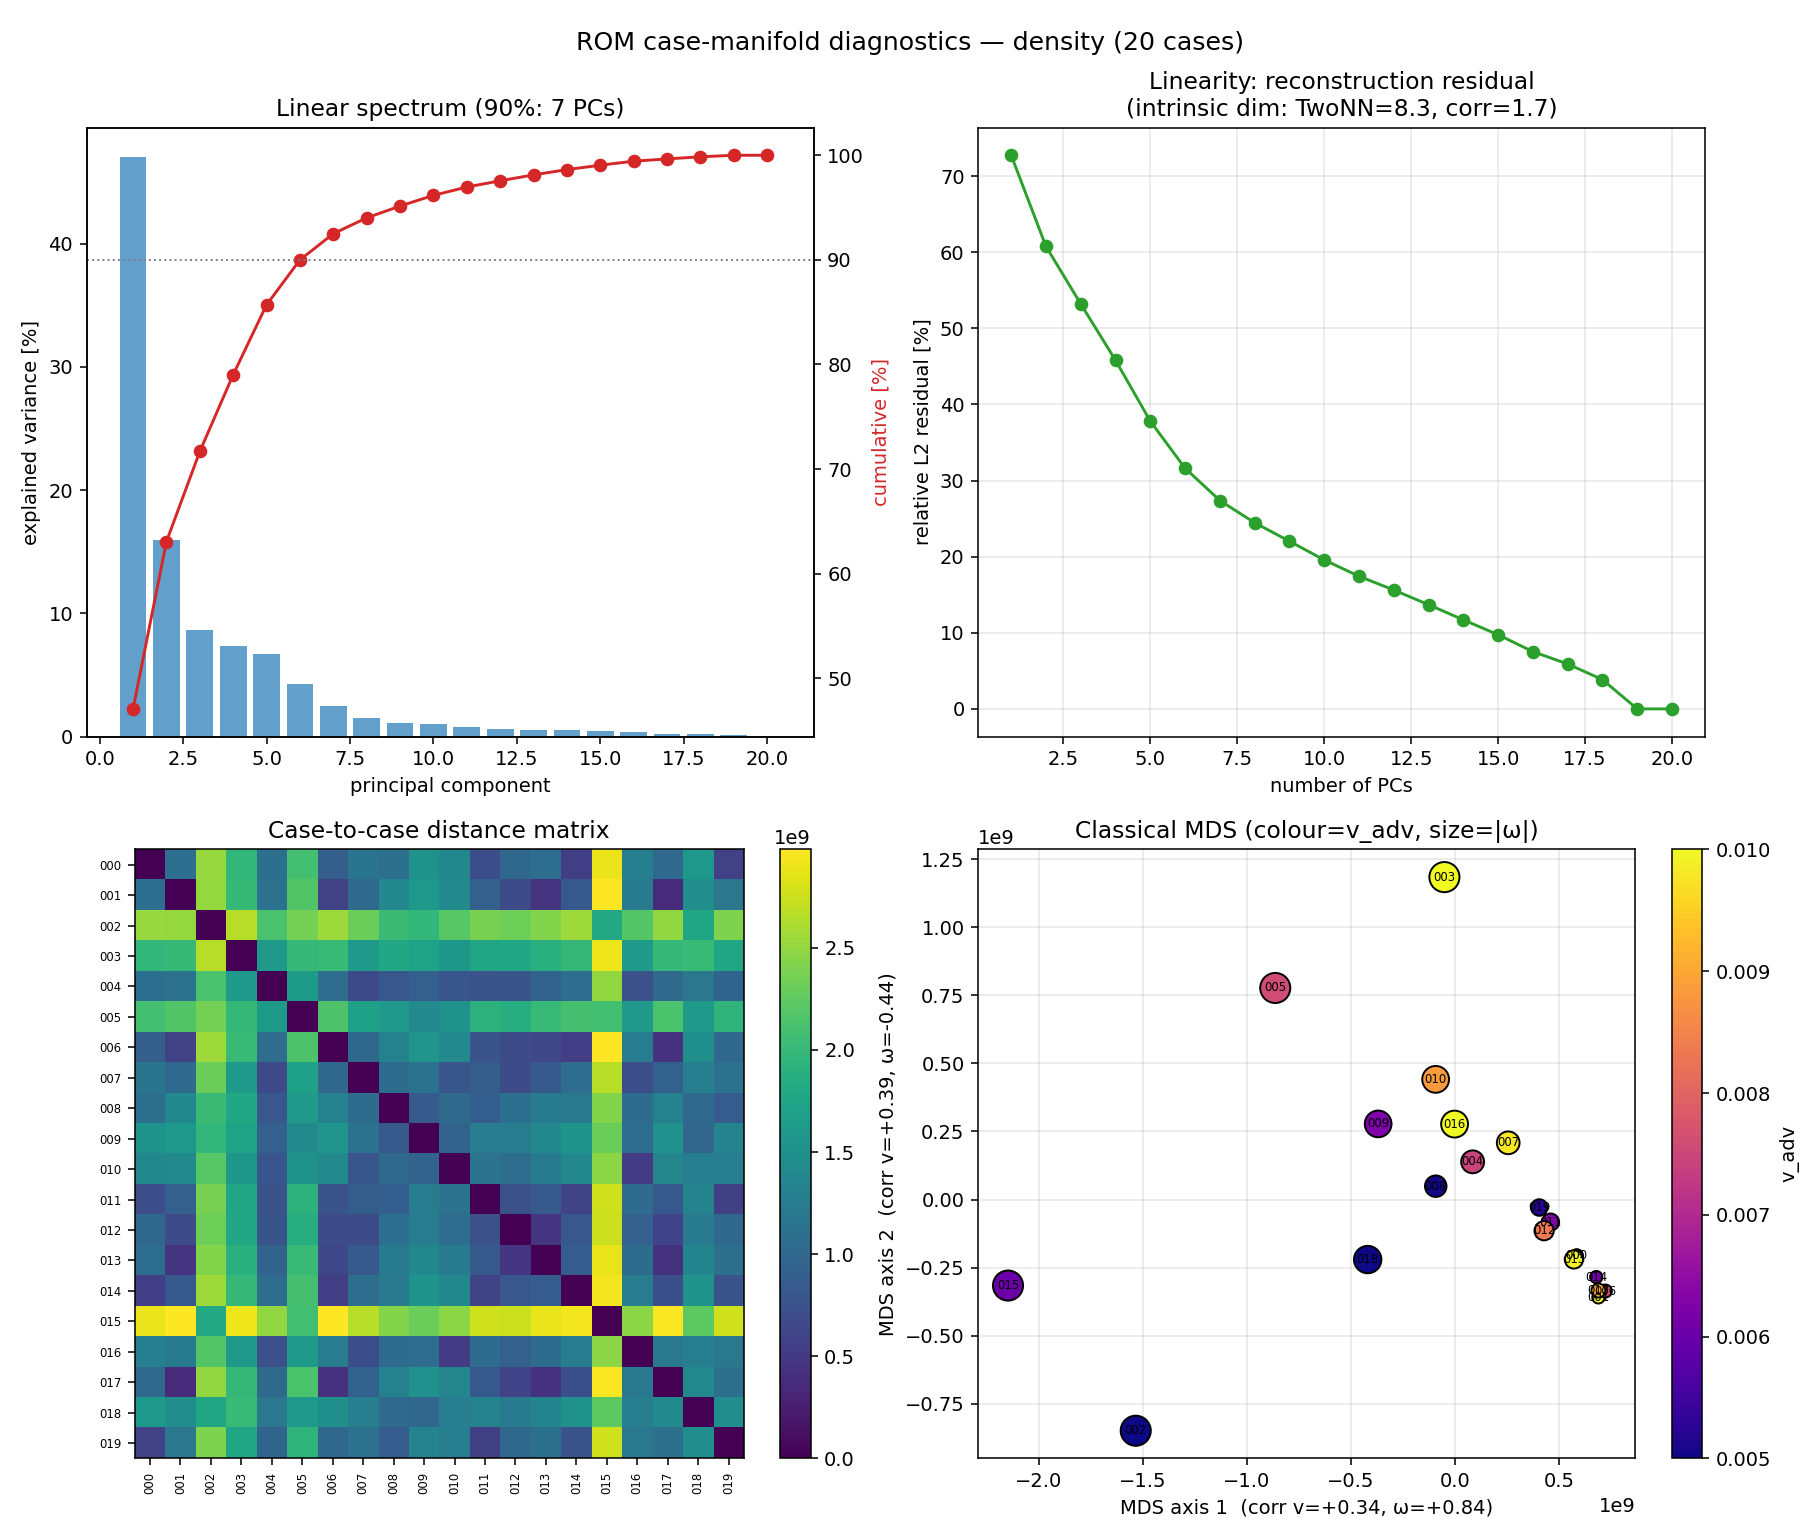
\includegraphics[width=0.9\linewidth]{rom_manifold_density_2d.png}
\caption{2D density case-manifold: intrinsic dim ${\approx}1.7$, a cleaner
and lower-dimensional manifold than 3D.}
\end{figure}

For \textbf{density}, integrating along $x$ averages out the
$\vadv$-driven wake variability and per-voxel noise (the spatial analogue
of the union's temporal denoising). For \textbf{particles}, $x$ is the
large, smooth, easily-predicted advection displacement; dropping it
removes the ``free'' mode and leaves only the small, chaotic in-plane stir
motion, which is harder to predict. So for the cloud, $x$ is signal, not
noise.

\paragraph{Caveat on the 2D ``improvement.''} Summing out $x$ is not a
free lunch: it reduces the predicted field's information content by
${\sim}300\times$. Part of the lower LOOCV error therefore reflects
predicting an \emph{easier, less-informative target} (the cross-section
integrates away exactly the $\vadv$-dependent wake the user may care
about), not only a genuinely better ROM. The 2D result is the right choice
\emph{if} the cross-section is the quantity of interest; it is not evidence
that the surrogate ``understands'' the full field better.

%======================================================================
\section{Summary of variants}
%======================================================================
\begin{table}[H]\centering\small
\begin{tabular}{llccl}
\toprule
target & variant & 90\% modes & best LOOCV & note \\
\midrule
density & union, full domain & 10 & 28.3\% & baseline (all 20) \\
density & union, near-pin $x$ & 11 & 24.4\% & drops the $\vadv$-wake \\
density & final-step & 12 & 49.3\% & time-avg far better \\
density & \textbf{2D $(y,z)$} & \textbf{6} & \textbf{20.6\%} & lowest error, but easier target \\
particles & 3D comoving & 11 & 36.1\% & harder than density \\
particles & 2D $(y,z)$ & 14 & 41.4\% & worse ($x$ is signal) \\
\midrule
\multicolumn{5}{l}{\emph{negative results (do not help):} weld-pitch inputs,
$\log$ inputs, first-stage ROM coeffs, richer regressors.}\\
\bottomrule
\end{tabular}
\caption{All main variants (rbf regressor, 20 cases). LOOCV = mean
held-out relative $L^2$ error.}
\end{table}

%======================================================================
\section{Conclusions and next steps}
%======================================================================
\begin{enumerate}
\item \textbf{Linear POD is a workable first approximation, not a validated
model of a linear response.} It gives ${\sim}21$--$28\%$ held-out density
error (per-case spread wide, e.g.\ $18$--$43\%$) --- useful as a baseline,
but the underlying manifold is \emph{curved} (intrinsic dimension
${\sim}2.5$ vs.\ ${\sim}10$ linear modes for 90\% energy). Linear POD works
here because it is a convenient global basis, not because the response is
linear; that mismatch is a real, not merely cosmetic, limitation.
\item \textbf{Both the basis and the regression are limited --- and both
point to more data.} The ${\sim}28\%$ held-out error is not purely a
regression failure: the linear POD \emph{basis} itself carries a
${\sim}10$--14\% error with no spectral elbow, because the curved ensemble
is not low-rank in a linear basis. The additional regression error is most
simply explained by degrees-of-freedom starvation (${\sim}7$--10
coefficients from 20 points). No information-free lever (normalization,
input features, regressor) helps, and all LOOCV numbers carry a standard
error of several points. Whether the residual error is \emph{specifically}
a boundary/extrapolation effect (Sec.~\ref{sec:curv}) is a plausible but
\emph{unconfirmed} hypothesis at $n{=}20$, not an established mechanism.
\item \textbf{Representation matters (within limits).} The
\emph{time-averaged} density is more predictable than a final snapshot, and
the \emph{2D $(y,z)$ cross-section} reaches ${\sim}21\%$ --- but the latter
also predicts a ${\sim}300\times$ smaller, lower-information target, so it
is a good choice only if the cross-section is the quantity of interest.
\item \textbf{More data is the prerequisite for everything else.} The
manifold is curved but smooth (no sharp folds), which is encouraging ---
but 20 points is too few to (i) fit the linear regression well, (ii)
confidently diagnose \emph{where} and \emph{why} the error concentrates, or
(iii) support any nonlinear alternative. Methods such as \emph{local /
patch POD}, \emph{manifold learning} (t-SNE, UMAP), and \emph{autoencoders}
would each overfit at $n{=}20$; they only become viable, and their value
only becomes testable, with substantially more samples (the literature
suggests ${\sim}50$--100 for a 2D parameter space of this complexity).
\end{enumerate}

\paragraph{Recommended next step.} \textbf{Acquire more samples}, and place
them to serve two goals at once: (a) \emph{extend and densify the sampling
envelope at its edges} (particularly the $\opin\approx-800$/low-$\vadv$
boundary, where the largest LOOCV errors sit), converting extrapolation
into interpolation; and (b) \emph{add samples where the curvature changes},
so the manifold's shape --- and hence the choice between linear POD, patch
POD, and nonlinear reduction --- can actually be resolved rather than
guessed. One suggestive (not conclusive) data point: adding the
previously-missing boundary case reduced the worst-case density error from
${\sim}48\%$ to ${\sim}43\%$; a larger, deliberately-placed batch is needed
to confirm the strategy and to unlock the nonlinear methods above.

%======================================================================
\section*{Reproducibility}
%======================================================================
All code is in the \texttt{jaxtrace/rom/} package (branch
\texttt{feature/rom-svd}), with drivers \texttt{run\_rom\_pca.py},
\texttt{run\_rom\_loocv.py}, \texttt{run\_rom\_particles.py},
\texttt{run\_rom\_first\_stage.py}, \texttt{run\_rom\_manifold.py},
\texttt{run\_rom\_curvature.py}, and
\texttt{run\_rom\_density\_compare.py}. Density product and 2D projection
are selected via \texttt{-{}-density-filename} and
\texttt{-{}-project-2d sum}; particle 2D via \texttt{-{}-components y z}.
The companion Markdown report \texttt{docs/rom\_feasibility\_report.md}
contains the full step-by-step derivations and the complete figure set.

\end{document}
